\section{Agent}

\subsection{La fonction d'utilité}

Le fonction d'utilité est une fonction permettant d'exprimer le "niveau de satisfaction" d'un agent en relation à une combinaison de consommation. Mais son utilité principale est celle d'exprimer les\textbf{ préférences d'un agent}.

\subsection{Les taux marginaux}
Une notion essentielle est celle de taux marginal, il représente analytiquement la dérivée d'une fonction. En microéconomie elle va nous informer sur l'utilité d'un échange ou non. L'axiome de convexité implique que si la consommation d'une quantité augmente son taux marginal diminue. \\
Cette dernière propriété nous permet d'interpréter les rapports de taux, si un rapport de taux est très élevé on a grand intérêt à consommer la ressource dont le taux marginal est au numérateur si l'on veut augmenter notre satisfaction (on verra ensuite que le choix optimal se réalise quand les rapports de taux sont égaux au rapports de prix).

\subsection{Programme de l'agent}
$$
\left\{
\begin{array}{cc}
 max_{C_i}U= & F(C_1,..,C_2)  \\
 sc: & \\
 & \sum_i p_i C_i \leq W \\
 & 0\leq C_i \ \forall i \in \{ 1,..n .\}
\end{array} 
\right.
$$
Les contraintes budgétaires dépendent des ressources et des emplois. Les ressources peuvent être par exemple les dotations initiales.
La résolution de ce programme nous donne $TMS_{i,j}=\frac{p_j}{p_i}$

\subsection{La demande}

La demande s'exprime comme $C_i=F(W,p_1,..,p_n)$

On l'obtiens à partir des conditions d'optimalité obtenues à l'aide du programme antérieur. Dans le cas de solutions intérieures la condition s'impose sur:
\begin{itemize}[label=\ding{69}]
\item \textbf{le taux marginal}: $TMS_{i,j}=\frac{p_j}{p_i}$. Dans le cas d'une Cobb-Douglass les solutions sont intérieures ce que l'on comprend en analysant la forme de la fonction (figure 1).
\newpage
\begin{figure}[h]
\begin{center}
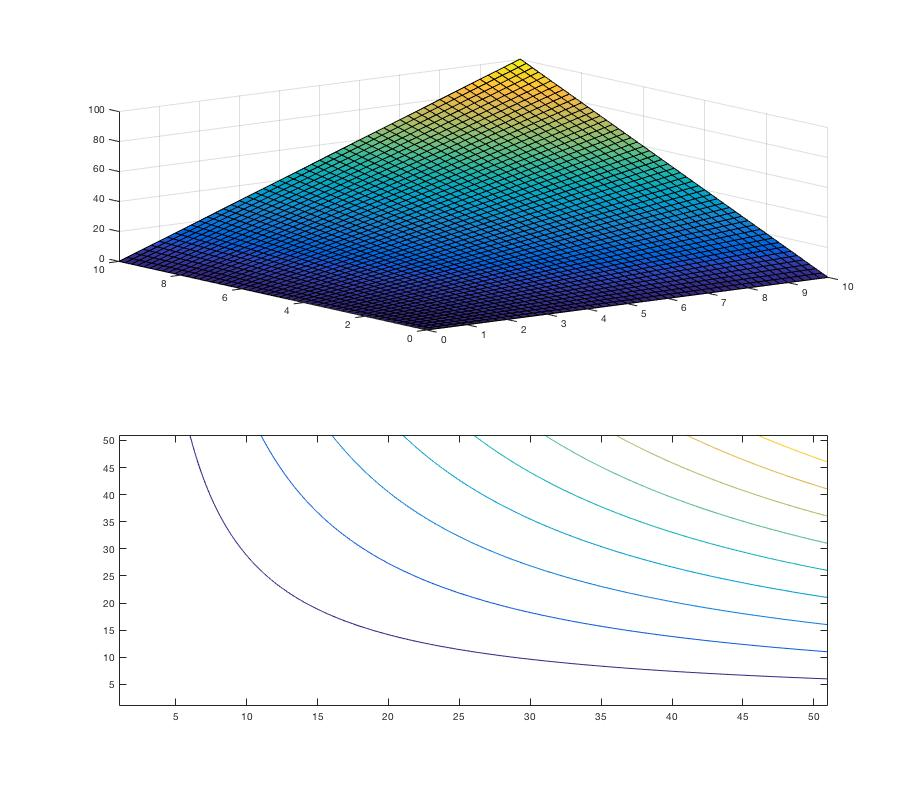
\includegraphics[scale=0.3]{./img/IM1}
\caption{surface Z=XY; Cobb Douglass avec $\alpha =1 ,\beta = 1$}
\end{center}
\end{figure}

Il est clairement plus rentable de tendre vers une solution intérieure. En raisonnant plus analytiquement on peut analyser les variation du TMS sur les coins et on observe que 
$$ TMS \in  \{ 0,\infty \} , \forall C_i \in \partial \Omega $$

\item \textbf{La saturation} de la contrainte budgétaire $\sum_i p_i C_i = W$

\end{itemize}
